
\documentclass{InsightArticle}

\usepackage{graphicx}
\usepackage[dvips,
bookmarks,
bookmarksopen,
backref,
colorlinks,linkcolor={blue},citecolor={blue},urlcolor={blue},
]{hyperref}


\title{ImageCalculator}

\release{1.00}

\author{Vamsi K. Jammalamadaka , Hans J. Johnson}
\authoraddress{The University of Iowa}

\begin{document}
\maketitle

\ifhtml
\chapter*{Front Matter\label{front}}
\fi


\begin{abstract}
\noindent
ImageCalculator is a command line program for doing simple mathematical operations to a series of images and generating an new output image and basic statistics about the output image.  The program uses the Insight Toolkit (www.ITK.org) for file IO and computations, and can operate on any of the image types supported by that library.
\end{abstract}

\tableofcontents

\section{Description}

ImageCalculator is a versitile program can perform arithmetic operations on a pixel by pixel basis across a series of 2D or 3D images, and generate basic statistics about the output image.
The general strategy for processing images is to do input filter on each image, apply a mathematical operation between each loaded image and an accumulator buffer, and finaly apply an output filter to the accumulator buffer before writing (See Fig.~\ref{fig:ImageCalculator}).

\begin{figure}
\begin{center}
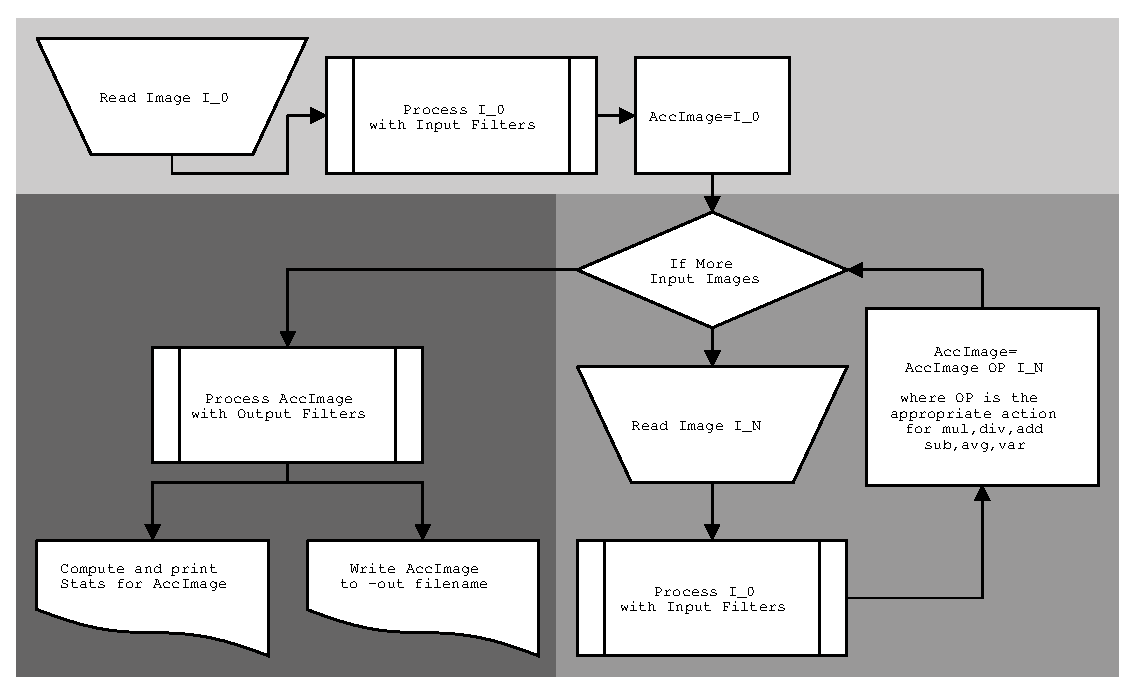
\includegraphics[width=6.0in]{figs/ImageCalculator.eps}
\end{center}
\caption{General strategy for consolidating information from a set of images}
\label{fig:ImageCalculator}
\end{figure}

The program can do the following tasks
\begin{itemize}

\item  Add , subtract, multiply, divide a set of images.
\item  Make an average image from a set of images.
\item  Make a variance image from a set of images.
\item  Add, subtract, multiply or divide a scalar value to the input images before performing other operations.
\item  Add, subtract, multiply or divide a scalar value from the output image before writing it out.
\item  It can print the following stats for the output image :-
       Average Image value, Sum of Image Values, Variance of Images, maximum \&
         minimum of an image and number of Pixels in an image.
\item If we input a mask, all the above statisticss will be calculated in the area covered by the mask.
\end{itemize}

Any number of images can be given as inputs to this program with the constraint that they must be of the same dimension and resolution.

User can specify the input pixel type in which all the arithmetic operations will be performed and output pixel type to write the image to a file.
The program supports unsigned char, short, unsigned short, integer, unsigned integer, float, double data types. ITK Metacommand utility is used to read in the images and arithmetic , statistical operations and other arguments specified by the user.

All the functions are templated over dimension and pixel type. The functions are called based on the user specified dimension and Input Image Pixel type.
The functions are in 3 header files\\1. Imgmath.h contains the arithmetic functions. ITK filters like AddImageFilter , SubtractImageFilter , DivideImageFilter , MultiplyImageFilter are used for performing the arithmetic. \\2. ImageCalculatorTemplates.h has templated functions to read in the series of input images process them by calling the arithmetic functions from Imgmath.h and write the output images. It also contains functions to perform Image statistics and  scalar arithmetic. \\3. ImageCalculatorUtils.h contains functions for printing the data types and comparing strings.\\

\section{Usage}

This program is called as:\\
ImageCalculator.exe $<$Required arguments$>$ [Optional Arguments]

Required Arguments:

\begin{itemize}

 \item -in  $<$ [number of inputs 'N'] filename1 filename2 ...filenameN $>$
       This is a list of Input Images. The list should be preceeded by the number of input images we are giving. Example: -in 3 Image1 Image2 image3
 \item -intype $<$DataType$>$
       Valid Input data types are: UCHAR SHORT USHORT INT UINT FLOAT DOUBLE.
 \item -Dimensions $<$dims$>$
       Input Dimension 2 or 3 should be specified.
\end{itemize}

Optional Arguments:

\begin{itemize}
\item -add
        Add Images.
\item -avg
        Make an average image
\item -div
        Perform Pixel wise division
\item -ifaddc $<$Constant Float$>$
        Add a constant number to Input Image after reading
\item -ifdivc $<$Constant Integer$>$
        Divide Input Images by constant integer after reading
\item -ifmulc $<$Constant Float$>$
        Multiply Input Images by constant  integer after reading
\item -ifsqr
        Square Input Images after reading
\item -ifsqrt
        Square Root of Input Images after reading
\item -ifsubc $<$Constant Float$>$
        Subtract constant integer from Input Images after reading
\item -ifbin
        Make a binary image from the Input Image
\item -ifgaussiansigma $<$Constant Float$>$
        Gaussian smooths Input Image after reading
\item -ifhisteq $<$Constant Integer$>$
        Equalizes every image to the current accumulator buffer.
\item -mul
        Multiply the Input Images
\item -ofaddc $<$Constant Float$>$
        Add constant integer to Output Image before writing
\item -ofdivc $<$Constant Float$>$
        Divide Output Image by constant number  before writing
\item -ofmulc $<$Constant Float$>$
        Multiply Output by constant number  before writing
\item -ofsqr
        Square Output Image before writing
\item -ofsqrt
        Square Root of Output Image before writing
\item -ofsubc $<$Constant Float$>$
        Subtract constant integer from Output Image before writing
\item -ofgaussiansigma $<$Constant Float$>$
        Gaussian smooths output Image after reading
\item -ofbin
        Make a binary image from the Output Image
\item -out
        Accumulator Image Should be output as floating point image

\item -outtype $<$DataType$>$
        Output image type. Image is written to the file in this type.

Valid Output data types are: UCHAR SHORT USHORT INT UINT FLOAT DOUBLE.
\item -statAMN
    Absolute minimum of Pixels in the Image
\item -statAMX
        Absolute maximum of Pixels in the Image
\item -statAVG
        Average Output Image Value
\item -statMAX
        Maximum of Pixels in the Image
\item -statMIN
        Minimum of Pixels in the Image
\item-statNPX
        Number of Mask Pixels
\item -statSUM
        Sum of output Image Values
\item -statVAR
        Variance of output Image
\item -statallcodes
        Prints the statistic flags and their description
\item -statmask $<$File Name$>$
        Image to mask against. If an image is given all the above statistics are calculated for the image under mask for a given statmaskvalue.
\item -statmaskvalue $<$Integer$>$
      If a mask image is given then we should specify an integer. Statistics are calculated for image under the mask having this value.
\item -sub
        Use Subtract op
\item -var
        make a variance image
\end{itemize}


\section{Examples}

This section provides some examples on using the program.

\begin{itemize}
\item Example1

Multiply two 2D images and taking the statistics of the output image.We specify the input data type as float in this example and the output type is not specified. The output will be written in input data type as the output is not specified.

Command:

{\bf ImageCalculator.exe -in 2 Image1.jpg Image2.jpg  -intype UCHAR  -mul -out Temp.jpg -Dimensions 2 -statNPX -statMIN -statAVG -statMAX -statVAR �statSUM
}

\item Example2

Subtracting two 3D images and write the binary output image.In this example all the operations are done in float data type and the output is written as Unsigned Character.

Command:

{\bf ImageCalculator.exe -in 2 Image1.hdr Image2.hdr  -intype FLOAT -outtype UCHAR -sub -out Temp.hdr -Dimensions 3 -ofbin}


\item Example3

Add six 3D images multiply the input image pixels by 10 before adding and divide the output image pixels by 5.  This example demonstrates that the program can take any number of inputs and we can perform scalar arithmetic on input and output image pixels.

Command:

{\bf ImageCalculator.exe -in 6 Image1.hdr Image2.hdr Image3.hdr Image4.hdr Image5.hdr Image6.hdr  -intype UCHAR -add -ifmulc 10 -ofdivc 5 -out Temp.hdr -Dimensions 3}


\end{itemize}

\section{Testing}

In this section we explain the tests which have been  included our CMakeLists.txt. The first 2 tests are for 2d images and the next 2 tests are performed on 3d images. In the source directory there is a folder named �TestImages� which contains some simple 2d and 3d images to do these tests.

In these tests we perform some functions with ImageCalculator and create a temporary image (Test.png for 2d; Test.hdr for 3d). This image is compared with the standard images in 'TestImages' folder to validate the result.
Comparision of images is done with ImageCompare program in ITK.

\begin{itemize}
\item Test1

We demonstrate 2d image addition in this test.
In the TestImage folder we have
UpperHalfHundreds.png , a 20x 20 image which contains upper half of its pixel values equal to 100.
LowerHalfHundreds.png , a 20x20 image which contains lower half of its pixel values equal to 100.
We add the 2 of them to get pixel values 100 at all locations.

 Test Command:

{\bf ImageCalculator.exe -in 2 UpperHalfHundreds.png LowerHalfHundreds.png  -intype UCHAR -outtype UCHAR -add -out Test.png -Dimensions 2 -statNPX -statMIN -statAVG -statMAX -statVAR �statSUM
}

The resultant statistics are.
AVG: 100, MAX: 100, MIN: 100, NPX: 400, SUM: 40000, VAR: 0

To verify we compare the result with the AllHundreds.png in the TestImage folder.

\item Test2

In this we see that we can add more than 2 inputs. ImageCalculator can take any number of inputs but in this example we add 5 images. We set the input Pixel Type as unsigned short and output as unsigned char for this example.

Test Command:

{\bf  ImageCalculator.exe -in 5 AllHundreds.png AllHundreds.png AllHundreds.png AllHundreds.png AllHundreds.png  -intype USHORT -outtype UCHAR -add -out Test.png -Dimensions 2 -statNPX -statMIN -statAVG -statMAX -statVAR -statSUM }

We get the output statistics as
AVG: 500, MAX: 500, MIN: 500, NPX: 400, SUM: 200000, VAR: 0,

ImageCalculator provides scalar arithmetic operations on images.
We can get the same result with scalar mutltiplication of AllHundreds.png.The test command for this scalar multiplication of the output image is(Output image is AllHundreds.png which we get by adding the UpperHalfHundreds.png and LowerhalfHundreds.png. See Test1 )\\
ImageCalculator.exe -in 2 UpperHalfHundreds.png LowerHalfHundreds.png  -intype USHORT -outtype UCHAR -add -out Temp.png -Dimensions 2 -ofmulc 5

The resultant image should have pixel values of 500 at all its locations.

To verify we compare the result with AllFiveHundreds.png

\item Test3

In this test we compare the 3d images. We divide a 5,5,5 image having all its pixels values 200 from another image with all pixel values 100. We should get all the pixel values equal to 2. The operations are performed with float data types.

Test Command:

{\bf ImageCalculator.exe -in 2 TwoHundred.hdr Hundred.hdr -intype FLOAT -outtype UCHAR -div -out Test.hdr -Dimensions 3 }

We should get an image having pixel value of 2 at all locations
To verify we compare the result with AllTwos.hdr



\item Test4

In this test we perform a simple scalar multiplication on a 3d image and verify its results.

Test Command:

{\bf ImageCalculator.exe -in 1 Hundred.hdr -intype UCHAR -out Test.hdr -Dimensions 3 -statNPX -statMIN -statAVG -statMAX -statVAR -statSUM -ofmulc 2}

This should result in an image having all its pixels equal to 200


We validate the result by comparing it to TwoHundred.hdr which has all pixels 200


\end{itemize}


\section{Further Information}

For further information we refer to the program source code, which is well documented.

\end{document}

